\chapter{Корреляции в модели Изинга, среднее поле и спонтанная намагниченность}

\lectureoverview{Одномерная цепь Изинга допускает точное решение, если заменить спины в узлах переменными связей. Эта замена переменных превращает статистическую сумму в произведение и показывает, что всякая корреляция при конечной температуре экспоненциально убывает. Решётки большей размерности ведут себя иначе, потому что каждый спин получает информацию от многих соседей. Если рассматривать их совместное влияние как среднее поле, получаются уравнение самосогласованности, критическая температура в приближении среднего поля и точное описание того, как сколь угодно малое внешнее поле выбирает одну намагниченную фазу.}

\section{Что на самом деле нашёл Изинг}

Исторический момент следует сформулировать точно. Ernst Ising решил одномерную модель, поставленную ему Wilhelm Lenz, и правильно установил отсутствие фазового перехода при конечной температуре. Чрезмерным был вывод о том, что то же заключение должно выполняться при любой размерности. Это не так. Уже двумерная модель имеет упорядоченную низкотемпературную фазу.

Для нашей нынешней цели точное решение в более высокой размерности — слишком амбициозная задача. Физически наглядного приближения будет достаточно, чтобы выявить переход, когда у каждого спина много соседей. Однако, прежде чем вводить это приближение, стоит точно решить одномерную цепь. Контраст между точным одномерным ответом и приближением для высокой размерности выявляет механизм, которого одному измерению недостаёт.

Фазовый переход здесь означает нечто большее, чем постепенное усиление уже имеющегося предпочтения. Когда температура проходит через критическое значение, равновесное состояние приобретает новое макроскопическое свойство: ненулевая намагниченность может сохраняться даже после того, как внешнее поле, использованное для ориентации образца, убрано. Поэтому расчёт должен ответить на 2 отдельных вопроса. Сохраняет ли удалённый спин память об ориентации выбранного спина, и может ли бесконечно малое поле упорядочить сколь угодно большой образец?

\section{Один спин как многократно используемый базовый элемент}

Рассмотрим двухсостоящую переменную
\begin{equation}
\sigma=\pm1,
\end{equation}
и выберем следующее соглашение для энергии:
\begin{equation}
E(\sigma)=-J\sigma,
\qquad J>0.
\end{equation}
Состояние \(\sigma=+1\) тогда имеет меньшую энергию. Параметр \(J\) может обозначать магнитный момент, умноженный на приложенное поле, но в этот расчёт входит только их произведение.

Будем рассматривать этот спин как малую подсистему, находящуюся в тепловом равновесии со всем остальным. Его статистическая сумма равна
\begin{align}
z
&=\sum_{\sigma=\pm1}e^{-\beta E(\sigma)}
 =\sum_{\sigma=\pm1}e^{\beta J\sigma} \\
&=e^{\beta J}+e^{-\beta J}
 =2\cosh(\beta J).
\end{align}

Тот же результат можно было бы встроить в совокупность из \(N\) независимых спинов. Полная статистическая сумма была бы просто \(Z=z^N\), так что \(\log Z=N\log z\), и всякая экстенсивная термодинамическая величина была бы в \(N\) раз больше своего односпинового значения. Такая точка зрения на подсистему заменяет более длинный комбинаторный подсчёт того, сколько спинов направлено вверх и вниз, но содержит ту же информацию.
Средняя энергия получается из логарифмической производной:
\begin{align}
\expect{E}
&=-\frac{\partial}{\partial\beta}\log z \\
&=-J\frac{\sinh(\beta J)}{\cosh(\beta J)}
 =-J\tanh(\beta J).
\end{align}
Так как \(E=-J\sigma\),
\begin{equation}
\expect{\sigma}=\tanh(\beta J).
\end{equation}

\begin{figure}[ht]
\centering
\includegraphics[width=0.80\textwidth]{lecture_09_figure_02.png}
\caption{Энергия и намагниченность одного спина, записанные в форме через гиперболический тангенс.}
\lectureframe{00:10:06}
\end{figure}

Эта единственная формула охватывает оба температурных предела. При низкой температуре \(\beta J\gg1\), и спин почти наверняка находится в состоянии с меньшей энергией. При высокой температуре \(\beta J\ll1\), так что
\begin{equation}
\expect{\sigma}\simeq \beta J\longrightarrow0.
\end{equation}
Тепловое возбуждение стирает энергетическое предпочтение.

\begin{classroomqa}
\audiencequestion{Должна ли средняя энергия иметь знак минус?}
\lecturerresponse{Да. Термодинамическое тождество имеет вид \(\expect{E}=-\partial_\beta\log z\), поэтому результат равен \(-J\tanh(\beta J)\). Деление на множитель \(-J\) в \(E=-J\sigma\) тогда даёт положительную намагниченность \(\expect{\sigma}=\tanh(\beta J)\). \lecturetimestamp{00:09:15--00:09:44}}
\end{classroomqa}

\section{Одномерная цепь}

Разместим \(N\) спинов в открытой цепи и введём взаимодействие соседних спинов:
\begin{equation}
H=-J\sum_{i=1}^{N-1}\sigma_i\sigma_{i+1},
\qquad \sigma_i=\pm1.
\label{eq:ising-chain}
\end{equation}
При \(J>0\) параллельная пара даёт вклад \(-J\), тогда как антипараллельная пара даёт вклад \(+J\). Поэтому 2 основных состояния таковы:
\begin{equation}
(+,+,\ldots,+)
\qquad\text{and}\qquad
(-,-,\ldots,-).
\end{equation}

\begin{figure}[ht]
\centering
\includegraphics[width=0.80\textwidth]{lecture_09_figure_03.png}
\caption{Гамильтониан открытой цепи и соответствующая больцмановская сумма.}
\lectureframe{00:19:15}
\end{figure}

Замена \(J\) на \(-J\) благоприятствует чередованию спинов. В открытой цепи или в периодической цепи чётной длины переопределение
\begin{equation}
\widetilde{\sigma}_i=(-1)^i\sigma_i
\end{equation}
преобразует антиферромагнитный знак обратно в ферромагнитный. Различие физически существенно, но алгебра статистической суммы в одном измерении остаётся той же. Периодическая цепь нечётной длины — известное исключение, потому что она не может чередоваться без фрустрации.

\begin{classroomqa}
\audiencequestion{Есть ли в гамильтониане цепи внешнее магнитное поле?}
\lecturerresponse{Пока нет. Уравнение~\eqref{eq:ising-chain} содержит только взаимодействие ближайших соседей. Однородное внешнее поле будет добавлено позже отдельным членом, \(-h\sum_i\sigma_i\), именно для того, чтобы проверить, как упорядоченное состояние реагирует на сколь угодно малую асимметрию. \lecturetimestamp{00:18:54--00:19:13}}
\end{classroomqa}

\subsection{Память как корреляционная функция}

Предположим, известно, что \(\sigma_i\) направлен вверх. Влияет ли эта информация на спин, удалённый на \(r\) связей? Диагностической величиной служит
\begin{equation}
C(r)=\expect{\sigma_i\sigma_{i+r}}.
\end{equation}
Если \(C(r)\) стремится к ненулевому числу при \(r\to\infty\), система сохраняет дальнюю память. Если же она стремится к нулю, влияние первого спина в конце концов исчезает.

Правильную интуицию даёт игра в испорченный телефон. Каждый человек передаёт следующему один двоичный символ. Если каждая передача безошибочна, исходный бит сохраняется сколь угодно долго. Если на каждом шаге есть хоть какая-то ненулевая вероятность ошибки, при многократной передаче исходное сообщение в конце концов теряется. Нулевая температура — это предел идеальной передачи для цепи Изинга. При любой положительной температуре между соседями возможны случайные несовпадения.

Для численной иллюстрации предположим, что вероятность правильной передачи за один шаг равна \(0.99\). Две безошибочные передачи происходят с вероятностью \(0.99^2=0.9801\), и каждый дополнительный шаг даёт ещё один множитель \(0.99\). Уже сто шагов делают ошибки обычными; десять тысяч шагов стирают память на практике. В цепи Изинга используется не эта вероятность отсутствия ошибки, а знаковая мера согласованности, но идея мультипликативной потери остаётся той же.

После различения вероятности и корреляции аналогия становится точной. Если \(p\) — вероятность того, что соседние спины совпадают, то
\begin{equation}
\expect{\sigma_i\sigma_{i+1}}
=p-(1-p)=2p-1.
\end{equation}
Таким образом, от связи к связи перемножается избыток согласованности \(2p-1\), а не само \(p\).

\section{Переменные на связях и точная статистическая сумма}

Решающая замена переменных состоит в том, чтобы описывать не отдельные спины, а отношения между ними:
\begin{equation}
\mu_i=\sigma_i\sigma_{i+1},
\qquad i=1,\ldots,N-1.
\label{eq:bond-variable}
\end{equation}
Каждая переменная связи равна \(+1\) при совпадении и \(-1\) при несовпадении. Если первый спин фиксирован, связи определяют все последующие спины:
\begin{align}
\sigma_2&=\sigma_1\mu_1,\\
\sigma_3&=\sigma_1\mu_1\mu_2,\\
\sigma_{r+1}&=\sigma_1\prod_{k=1}^{r}\mu_k.
\end{align}
Избыточности нет. Данные \((\sigma_1,\mu_1,\ldots,\mu_{N-1})\) эквивалентны \((\sigma_1,\ldots,\sigma_N)\).

В этих переменных энергия просто равна
\begin{equation}
H=-J\sum_{i=1}^{N-1}\mu_i.
\end{equation}
Взаимодействующие узловые переменные превратились в независимые переменные связей. Суммирование сначала по двум значениям \(\sigma_1\) даёт
\begin{align}
Z_N
&=2\sum_{\{\mu_i=\pm1\}}
\exp\left(\beta J\sum_{i=1}^{N-1}\mu_i\right)\\
&=2\prod_{i=1}^{N-1}
\left(\sum_{\mu_i=\pm1}e^{\beta J\mu_i}\right)\\
&=2\left[2\cosh(\beta J)\right]^{N-1}.
\label{eq:chain-partition}
\end{align}
Множителей \(N-1\), потому что открытая цепь из \(N\) узлов имеет \(N-1\) связей.

Начальный множитель 2 — это глобальный выбор первого спина. Он даёт лишь \(\log2\) в \(\log Z_N\), тогда как связи дают член, пропорциональный \(N-1\). Этот множитель важен для точного счёта при конечном размере, но исчезает из плотности свободной энергии при \(N\to\infty\). Поэтому на доске его могли назвать «несущественным», фактически не отбрасывая.

\begin{figure}[ht]
\centering
\includegraphics[width=0.82\textwidth]{lecture_09_figure_04.png}
\caption{Гамильтониан по узлам, переписанный как сумма по независимым связям, и полученная факторизованная статистическая сумма.}
\lectureframe{00:35:35}
\end{figure}

\begin{classroomqa}
\audiencequestion{Куда делась сумма в показателе экспоненты, когда окончательный ответ превратился в степень?}
\lecturerresponse{Она превратилась в произведение, прежде чем превратиться в степень:
\[
e^{\beta J\sum_i\mu_i}=\prod_i e^{\beta J\mu_i}.
\]
Сумма по всем конфигурациям связей затем распадается на одну сумму из 2 членов для каждой связи. Поскольку каждый множитель равен \(2\cosh(\beta J)\), произведение есть эта величина в степени \((N-1)\). Если выписать 3 спина и 2 связи, факторизация становится совершенно явной. \lecturetimestamp{00:33:25--00:35:36}}
\end{classroomqa}

Это простое дуальное описание: связанные переменные на узлах заменены несвязанными переменными на связях. Слово \emph{дуальность} уместно, потому что одна и та же система имеет 2 описания с очень непохожими степенями свободы. Здесь это точная замена переменных для открытой одномерной цепи.

На языке решёток исходные переменные живут на вершинах, а новые переменные — на рёбрах. Глобальный выбор первого спина — та единственная дополнительная информация, которая нужна, чтобы восстановить вершины по рёбрам. Такой обмен узлы–связи — скромный пример схемы, которая в статистической механике более высоких размерностей становится гораздо более мощной.

\subsection{Согласованность ближайших соседей}

Для каждой связи распределение одинаково,
\begin{equation}
\begin{aligned}
\Pr(\mu=+1)&=\frac{e^{\beta J}}{2\cosh(\beta J)},\\
\Pr(\mu=-1)&=\frac{e^{-\beta J}}{2\cosh(\beta J)}.
\end{aligned}
\end{equation}
Следовательно,
\begin{equation}
\expect{\mu_i}
=\expect{\sigma_i\sigma_{i+1}}
=\tanh(\beta J).
\label{eq:nearest-correlation}
\end{equation}

\begin{figure}[ht]
\centering
\includegraphics[width=0.80\textwidth]{lecture_09_figure_05.png}
\caption{Корреляция ближайших соседей, выраженная как среднее значение переменной связи.}
\lectureframe{00:36:52}
\end{figure}

Следовательно, вероятность того, что соседние спины совпадают, равна
\begin{equation}
p_{\rm same}
=\frac{1+\tanh(\beta J)}{2}.
\end{equation}
При положительном \(J\) она превышает одну вторую, при нулевой температуре стремится к единице, а при бесконечной температуре становится равной одной второй.

\begin{classroomqa}
\audiencequestion{Почему положительная корреляция ближайших соседей означает, что спины предпочитают параллельную ориентацию, а не антипараллельную?}
\lecturerresponse{При \(J>0\) у связи с параллельными спинами энергия \(-J\), а у связи с антипараллельными — \(+J\). Положительное значение \(\expect{\mu}\) означает, что \(\mu=+1\), а значит, параллельная ориентация встречается чаще. Будет ли эффективная связь в реальном материале ферро- или антиферромагнитной, зависит от его микроскопической электронной структуры; принятое здесь соглашение о знаке описывает ферромагнетик. \lecturetimestamp{00:43:45--00:44:48}}
\end{classroomqa}

\begin{classroomqa}
\audiencequestion{Что происходит с этой корреляцией при очень высокой температуре?}
\lecturerresponse{Когда \(T\to\infty\), \(\beta\to0\) и \(\tanh(\beta J)\to0\). Тогда даже ближайшие соседи не несут информации друг о друге: состояние каждого спина фактически определяется случайным выбором. \lecturetimestamp{00:46:42--00:47:20}}
\end{classroomqa}

\subsection{Корреляция на больших расстояниях}

Для спинов, разделённых \(r\) связями,
\begin{align}
\sigma_i\sigma_{i+r}
&=\sigma_i
\left(\prod_{k=i+1}^{i+r-1}\sigma_k^2\right)
\sigma_{i+r}\\
&=(\sigma_i\sigma_{i+1})
(\sigma_{i+1}\sigma_{i+2})\cdots
(\sigma_{i+r-1}\sigma_{i+r})\\
&=\prod_{k=i}^{i+r-1}\mu_k.
\end{align}
Поскольку \(\mu_k\) независимы,
\begin{equation}
C(r)=\expect{\sigma_i\sigma_{i+r}}
=\left[\tanh(\beta J)\right]^r.
\label{eq:exact-correlation}
\end{equation}

\begin{figure}[ht]
\centering
\includegraphics[width=0.80\textwidth]{lecture_09_figure_06.png}
\caption{Промежуточные множители \(\sigma_k^2=1\) превращают произведение удалённых спинов в произведение независимых связей.}
\lectureframe{00:41:35}
\end{figure}

\begin{classroomqa}
\audiencequestion{Корреляционная функция содержит только два концевых спина. Откуда взялись все промежуточные спины?}
\lecturerresponse{Их вставили лишь как множители, равные единице: \(\sigma_k^2=1\). Попарное объединение соседних копий превращает произведение концевых спинов в переменные связи, а именно для них тепловое распределение факторизуется. Значение корреляционной функции от этого не меняется. \lecturetimestamp{00:41:41--00:42:26}}
\end{classroomqa}

При любой конечной температуре,
\begin{equation}
0<\tanh(\beta J)<1,
\end{equation}
поэтому память затухает экспоненциально. Запись
\begin{equation}
C(r)=e^{-r/\xi}
\end{equation}
определяет точную корреляционную длину
\begin{equation}
\xi^{-1}=-\log\!\left[\tanh(\beta J)\right].
\label{eq:correlation-length}
\end{equation}
Лишь при \(T=0\) величина \(\xi\) расходится. При низкой, но ненулевой температуре,
\begin{equation}
\xi\simeq \frac{1}{2}e^{2\beta J},
\end{equation}
поэтому цепочка может содержать очень длинные участки с одинаково ориентированными спинами, не обладая при этом истинным порядком бесконечного радиуса действия.

Поэтому цепочка выглядит сгруппированной в домены. Видны длинная серия спинов, направленных вверх, затем переключение, затем длинная серия спинов, направленных вниз, затем ещё одно переключение. Низкая температура делает эти серии длинными, потому что доменная стенка редка; однако совсем доменные стенки не исчезают. Для намагниченности нужна бесконечная длина памяти, а не просто очень большая.

\section{Почему большее число соседей меняет задачу}

Одно измерение не обеспечивает исправления ошибок. Как только одна связь оказывается несогласованной с предыдущей, у следующего спина нет независимого источника, который подсказал бы, какая ориентация предполагалась. Поэтому цепочка состоит из длинных выровненных доменов, разделённых редкими переключениями.

В квадратной решётке у каждого узла 4 ближайших соседа. В кубической — 6. На \(d\)-мерной гиперкубической решётке у него
\begin{equation}
z=2d
\end{equation}
ближайших соседей. Узел, получающий 3 согласующихся сообщения и 1 несогласующееся, может следовать большинству. Окружение из многих соседей подавляет изолированные ошибки почти так же, как избыточные сообщения позволяют исправлять ошибки.

Если среднее значение спина у соседей равно \(m\), то их сумма имеет среднее \(zm\). Её обычная флуктуация имеет порядок \(\sqrt{z}\), так что вдали от \(m=0\) относительная флуктуация масштабируется приблизительно как
\begin{equation}
\frac{\sqrt{z}}{z|m|}
=\frac{1}{\sqrt{z}\,|m|}.
\end{equation}
Вот почему среднее поле становится правдоподобным при большом координационном числе. Это также предупреждает, что аппроксимация наименее надёжна вблизи критической точки, где \(m\) мало.

Эту интуицию больших чисел передаёт запоминающееся изречение: сто независимых голосов вряд ли ошибутся в одном и том же направлении. Количественная версия — закон квадратного корня. Согласованное смещение в \(z\) переменных пропорционально \(z\), тогда как случайное рассогласование обычно пропорционально лишь \(\sqrt{z}\). Поэтому увеличение размерности меняет не только число соседей, но и надёжность их коллективного сообщения.

\begin{classroomqa}
\audiencequestion{Соответствуют ли размерности выше трёх какому-нибудь физическому магнитному материалу?}
\lecturerresponse{Непосредственно — нет, если понимать их как пространственные размерности. Большое \(d\) — это решаемый предел, в котором у каждого узла много соседей и усреднение становится контролируемым. Когда механизм становится там виден, можно спросить, насколько далеко он сохраняется при переходе к физическим размерностям. Для модели Изинга уже двух измерений достаточно для перехода при конечной температуре, хотя среднее поле не даёт точного двумерного ответа. \lecturetimestamp{00:52:32--00:53:50}}
\end{classroomqa}

\section{Среднее поле как задача самосогласованности}

Рассмотрим один спин \(\sigma_i\). Его взаимодействие с его \(z=2d\) соседями описывается выражением
\begin{equation}
E_i=-J\sigma_i\sum_{j\in{\rm nn}(i)}\sigma_j.
\label{eq:local-energy}
\end{equation}
Пусть
\begin{equation}
m=\expect{\sigma}
\end{equation}
обозначает однородную намагниченность в расчёте на спин. В приближении среднего поля флуктуирующая сумма по соседям заменяется её средним значением:
\begin{equation}
\sum_{j\in{\rm nn}(i)}\sigma_j
\longrightarrow zm=2dm.
\end{equation}
Тогда выделенный спин имеет эффективную односпиновую энергию
\begin{equation}
E_i^{\rm MF}=-2dJm\,\sigma_i.
\label{eq:mean-field-energy}
\end{equation}

\begin{figure}[ht]
\centering
\includegraphics[width=0.82\textwidth]{lecture_09_figure_07.png}
\caption{Выбранный спин, его \(2d\) ближайших соседей и замена их суммы средней намагниченностью.}
\lectureframe{01:00:30}
\end{figure}

Теперь можно вновь использовать результат для одного спина с эффективным полем \(2dJm\):
\begin{equation}
\expect{\sigma_i}_{\rm effective}
=\tanh(2\beta dJm).
\end{equation}
Но выбранный узел ничем не особенный. Трансляционная инвариантность требует, чтобы его среднее совпадало с предполагаемым средним \(m\). Следовательно,
\begin{equation}
\boxed{m=\tanh(2\beta dJm)}.
\label{eq:self-consistency}
\end{equation}
Вот почему среднее поле также называют приближением самосогласованного поля: намагниченность, создающая эффективное поле, должна совпадать с намагниченностью, порождаемой этим полем.

\begin{classroomqa}
\audiencequestion{Не отсутствует ли в ответе для эффективного одного спина множитель \(\beta\)?}
\lecturerresponse{Он должен присутствовать. Аргумент экспоненты или гиперболического тангенса безразмерен, поэтому эффективная энергия \(2dJm\) входит как \(2\beta dJm\). \lecturetimestamp{01:00:13--01:00:27}}
\end{classroomqa}

\begin{classroomqa}
\audiencequestion{Разве уравнение не утверждает просто, что \(m\) пропорционально самому себе?}
\lecturerresponse{Нет. Неизвестная намагниченность стоит внутри нелинейной функции:
\[
m=\tanh(2\beta dJm).
\]
Это неявное уравнение, и в зависимости от температуры оно может иметь одно или несколько решений. \lecturetimestamp{01:02:12--01:02:42}}
\end{classroomqa}

\begin{classroomqa}
\audiencequestion{Предполагает ли уравнение самосогласованности высокую температуру или малый аргумент гиперболического тангенса?}
\lecturerresponse{Нет. Уравнение \(m=\tanh(2\beta dJm)\) — это полное уравнение среднего поля при любой температуре. Лишь более позднее приближение, такое как \(\tanh x\simeq x\), требует малого \(x\), и оно используется вблизи критической точки, чтобы найти или разложить появляющееся решение. \lecturetimestamp{01:02:44--01:03:12}}
\end{classroomqa}

\begin{classroomqa}
\audiencequestion{Отличается ли обозначение с чертой сверху от обычного среднего в угловых скобках?}
\lecturerresponse{Нет. Черта, использованная на доске, — это сокращённая запись термического среднего: \(\bar{\sigma}=\expect{\sigma}=m\). \lecturetimestamp{01:03:19--01:03:42}}
\end{classroomqa}

\begin{classroomqa}
\audiencequestion{Все ли \(2d\) спинов являются ближайшими соседями, и дали бы связи большего радиуса аналогичный эффект?}
\lecturerresponse{На гиперкубической решётке — да: вдоль каждой из \(d\) координатных осей есть по 2 ближайших соседа. Связи со следующими ближайшими и более далёкими соседями задают другую модель и вообще имеют собственные константы, но увеличение радиуса взаимодействия тоже повышает эффективное координационное число и может сделать рассуждения среднего поля более точными. \lecturetimestamp{01:03:43--01:05:12}}
\end{classroomqa}

\section{Графическое представление фазового перехода}

Введём
\begin{equation}
K=2\beta dJ,
\qquad
y=Km.
\end{equation}
Тогда уравнение~\eqref{eq:self-consistency} принимает вид
\begin{equation}
\frac{y}{K}=\tanh y.
\label{eq:graph-equation}
\end{equation}
Правая часть — фиксированная сигмоида. Левая часть — прямая, проходящая через начало координат, с наклоном
\begin{equation}
\frac{1}{K}=\frac{T}{2dJ},
\end{equation}
где \(k_{\rm B}=1\).

При высокой температуре прямая крута и пересекает \(\tanh y\) только в точке \(y=0\). При низкой температуре прямая полога, и имеются 3 точки пересечения: \(y=0\) и симметричная пара \(y=\pm y_0\). Порог достигается, когда прямая и \(\tanh y\) имеют одинаковый наклон в начале координат. Поскольку \(\tanh'(0)=1\),
\begin{equation}
K_c=1,
\qquad
T_c^{\rm MF}=2dJ.
\label{eq:mean-field-tc}
\end{equation}
Это критическая температура в приближении среднего поля, а не точный ответ при малой размерности.

Предположение \(J>0\) говорит, что соседние спины предпочитают совпадать; оно не выделяет \(+m\) по сравнению с \(-m\). При нулевом внешнем поле гамильтониан не изменяется при глобальном перевороте \(\sigma_i\mapsto-\sigma_i\), поэтому две ненулевые точки пересечения физически эквивалентны. Выбор только положительной половины графика — это удобное графическое соглашение, а не потеря отрицательной фазы.

\begin{figure}[ht]
\centering
\includegraphics[width=0.82\textwidth]{lecture_09_figure_08.png}
\caption{Семейство прямых и \(\tanh y\): одна точка пересечения при высокой температуре и 3 — при низкой.}
\lectureframe{01:11:50}
\end{figure}

\begin{figure}[ht]
\centering
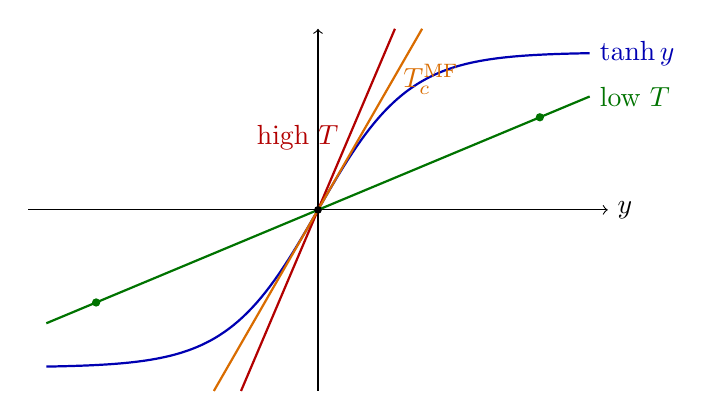
\begin{tikzpicture}[x=1.15cm,y=2.0cm]
\draw[->] (-3.2,0) -- (3.2,0) node[right] {$y$};
\draw[->] (0,-1.15) -- (0,1.15);
\draw[thick,blue!70!black,domain=-3:3,samples=120]
  plot (\x,{tanh(\x)}) node[right] {$\tanh y$};
\draw[thick,red!70!black] (-0.85,-1.15) -- (0.85,1.15)
  node[pos=0.70,left] {high \(T\)};
\draw[thick,orange!85!black] (-1.15,-1.15) -- (1.15,1.15)
  node[pos=0.86,right] {\(T_c^{\rm MF}\)};
\draw[thick,green!45!black] (-3,-0.72) -- (3,0.72)
  node[right] {low \(T\)};
\fill (0,0) circle (1.4pt);
\fill[green!45!black] (-2.45,-0.588) circle (1.5pt);
\fill[green!45!black] (2.45,0.588) circle (1.5pt);
\end{tikzpicture}
\caption{Нормированная реконструкция графического аргумента самосогласованности.}
\end{figure}

Ненулевая ветвь возникает непрерывно. Вблизи перехода,
\begin{equation}
\tanh(Km)=Km-\frac{(Km)^3}{3}+O(m^5).
\end{equation}
При \(K>1\) малые ненулевые решения удовлетворяют
\begin{equation}
m^2\simeq \frac{3(K-1)}{K^3}.
\end{equation}
Таким образом, приближение среднего поля предсказывает знакомое возникновение по закону квадратного корня \(m\propto(T_c-T)^{1/2}\).

Утверждение об устойчивости можно сформулировать и без опоры на то, как нарисован график. С точностью до не зависящей от \(m\) константы среднеполевая свободная энергия в расчёте на спин равна
\begin{equation}
f_{\rm MF}(m)
=dJm^2-\frac{1}{\beta}
\log\!\left[2\cosh(2\beta dJm)\right].
\label{eq:mf-free-energy}
\end{equation}
Условие стационарности имеет вид
\begin{equation}
\frac{\partial f_{\rm MF}}{\partial m}
=2dJ\left[m-\tanh(2\beta dJm)\right]=0.
\end{equation}
Выше \(T_c^{\rm MF}\) минимумом является \(m=0\). Ниже неё начало координат является локальным максимумом, а два ненулевых решения — вырожденными минимумами. Геометрия точек пересечения и термодинамика свободной энергии говорят об одном и том же.

\begin{classroomqa}
\audiencequestion{Решение \(m=0\) остаётся точкой пересечения ниже \(T_c^{\rm MF}\). Почему физической должна быть ненулевая ветвь?}
\lecturerresponse{Если повышать температуру, начиная с нуля, система уже оказывается на намагниченной ветви. Более формально, ниже перехода среднеполевая свободная энергия имеет минимумы при \(\pm m_0\), тогда как \(m=0\) становится максимумом. Бесконечно малое внешнее поле затем выбирает один из минимумов и устраняет кажущуюся неоднозначность. \lecturetimestamp{01:11:34--01:12:18}}
\end{classroomqa}

\section{Почему в одном измерении среднее поле не работает}

Подстановка \(d=1\) в уравнение~\eqref{eq:mean-field-tc} предсказала бы переход при \(T=2J\), что противоречит точному одномерному решению. Никакая алгебраическая величина не расходится. Приближение терпит неудачу, потому что два соседа не образуют большой статистической среды и потому что одномерные доменные стенки обладают необычно большой энтропией.

Начнём с состояния, в котором все спины направлены вверх. Разорванная связь меняет свою энергию с \(-J\) на \(+J\), так что каждая разорванная связь стоит
\begin{equation}
\Delta E_{\rm bond}=2J.
\end{equation}
На квадратной решётке один перевёрнутый спин разрывает четыре связи и стоит \(8J\). Два соседних перевёрнутых спина имеют периметр из шести разорванных связей и стоят \(12J\), тогда как два далеко разнесённых перевёрнутых спина разрывают восемь связей и стоят \(16J\).

\begin{figure}[ht]
\centering
\includegraphics[width=0.82\textwidth]{lecture_09_figure_09.png}
\caption{Два соседних перевёрнутых спина на квадратной решётке; их общая связь удовлетворена, так что остаётся граница из шести связей.}
\lectureframe{01:17:30}
\end{figure}

В двумерном случае компактная перевёрнутая капля поэтому требует энергии, пропорциональной длине её границы:
\begin{equation}
\Delta E_{\rm 2d}=2J\,|\partial D|.
\end{equation}
При росте капли её граница, как правило, тоже растёт.

В одном измерении всё иначе. Непрерывный перевёрнутый блок, какова бы ни была его длина, имеет только две доменные стенки:
\begin{equation}
\Delta E_{\rm 1d}=2(2J)=4J.
\label{eq:one-d-domain-cost}
\end{equation}

\begin{figure}[ht]
\centering
\includegraphics[width=0.82\textwidth]{lecture_09_figure_10.png}
\caption{Длинный перевёрнутый блок в одном измерении, ограниченный всего двумя доменными стенками.}
\lectureframe{01:19:10}
\end{figure}

Существует порядка \(N^2\) способов выбрать две стенки такого блока в цепочке из \(N\) узлов. Их энергия не растёт с увеличением расстояния между стенками. Поэтому при любой положительной температуре энтропия обеспечивает сколь угодно большие перевёрнутые домены. В двумерном случае энергия границы может при достаточно низкой температуре превзойти энтропию контуров. Эта конкуренция энергии и энтропии — геометрический факт, которого среднее поле не видит, когда рассматривает \(d=1\) и \(d=2\) всего лишь как разные численные значения одного и того же коэффициента.

\begin{classroomqa}
\audiencequestion{Требует ли постоянная цена двух стенок, чтобы перевёрнутые спины были соседними?}
\lecturerresponse{Да. Речь идёт об одном непрерывном перевёрнутом блоке. Если перевёрнутые спины образуют несколько разделённых блоков, каждый блок вносит две дополнительные доменные стенки. Важно то, что один блок может быть сколь угодно длинным, сохраняя при этом только две стенки. \lecturetimestamp{01:18:32--01:18:40}}
\end{classroomqa}

\begin{classroomqa}
\audiencequestion{Само среднеполевое уравнение, кажется, не показывает никакого качественного различия между \(d=1\) и \(d=2\). В этом и состоит проблема?}
\lecturerresponse{Именно. Среднее поле предсказывает переход для любого положительного \(d\), поэтому в одном измерении оно качественно неверно. При его выводе предполагалось много слабо флуктуирующих соседей, а геометрия доменных стенок была отброшена. Одномерный случай определяется точным решением по связям, а не среднеполевой подстановкой \(d=1\). \lecturetimestamp{01:19:44--01:20:28}}
\end{classroomqa}

\section{Внешнее поле выбирает фазу}

Добавим однородное поле \(h\), приняв соглашение, что \(h>0\) благоприятствует \(\sigma=+1\):
\begin{equation}
H=-J\sum_{\langle ij\rangle}\sigma_i\sigma_j
-h\sum_i\sigma_i.
\label{eq:ising-with-field}
\end{equation}
Среднеполевая энергия одного выделенного спина равна
\begin{equation}
E_i^{\rm MF}=-(2dJm+h)\sigma_i,
\end{equation}
и уравнение самосогласованности принимает вид
\begin{equation}
\boxed{m=\tanh\!\left[\beta(2dJm+h)\right]}.
\label{eq:self-consistency-field}
\end{equation}
При \(K=2\beta dJ\) и \(y=Km\),
\begin{equation}
\frac{y}{K}=\tanh(y+\beta h).
\label{eq:shifted-graph}
\end{equation}

\begin{figure}[ht]
\centering
\includegraphics[width=0.82\textwidth]{lecture_09_figure_11.png}
\caption{Член внешнего поля, добавленный в уравнение самосогласованности, и соответствующая сдвинутая графическая конструкция.}
\lectureframe{01:26:20}
\end{figure}

\begin{classroomqa}
\audiencequestion{Почему поле добавляется только внутри гиперболического тангенса? Не должно ли оно также изменить левую часть?}
\lecturerresponse{Левая часть — это предполагаемая намагниченность \(m\), или, что то же самое, \(y/K\). Правая часть — это намагниченность, вычисленная для спина в полном эффективном поле \(2dJm+h\). Самосогласованность приравнивает эти две величины. Если оставить \(y=Km\) в качестве определения, новый член появляется только в аргументе \(\tanh(y+\beta h)\). \lecturetimestamp{01:23:46--01:26:18}}
\end{classroomqa}

\begin{classroomqa}
\audiencequestion{Можно ли описать то же графическое изменение, перемещая прямые, а не сдвигая кривую \(\tanh\)?}
\lecturerresponse{Да. Можно оставить график \(\tanh y\) неизменным и переписать уравнение так, чтобы прямая имела ненулевой свободный член. Точки пересечения при этом те же самые. Эти два описания различаются только тем, какая сторона уравнения выбрана в качестве фиксированного графика. \lecturetimestamp{01:35:07--01:36:26}}
\end{classroomqa}

При \(h\neq0\) начало координат больше не является решением. Ниже \(T_c^{\rm MF}\) сколь угодно малое положительное поле выбирает положительную ветвь; отрицательное поле выбирает отрицательную ветвь.

\begin{figure}[ht]
\centering
\includegraphics[width=0.82\textwidth]{lecture_09_figure_12.png}
\caption{Слабое поле устраняет симметричную точку пересечения и выбирает одну намагниченную ветвь.}
\lectureframe{01:36:22}
\end{figure}

Корректная формулировка требует определённого порядка предельных переходов. Конечная система при точном \(h=0\) обладает симметрией относительно переворота спинов и потому имеет \(\expect{m}=0\) в полном равновесном ансамбле. Спонтанная намагниченность равна
\begin{equation}
m_{\rm sp}
=\lim_{h\to0^+}\lim_{N\to\infty}\expect{m}_{N,h},
\end{equation}
где термодинамический предел берётся первым. Изменение знака бесконечно малого поля даёт \(-m_{\rm sp}\). Полная разность полевой энергии пропорциональна \(Nh\), так что даже очень малое поле становится решающим для макроскопического образца.

Соответствующая свободная энергия наглядно показывает этот наклон:
\begin{equation}
f_{\rm MF}(m;h)
=dJm^2-\frac{1}{\beta}
\log\!\left[2\cosh\!\left(\beta(2dJm+h)\right)\right].
\end{equation}
При \(h=0\) две ямы имеют одинаковую глубину. Положительное \(h\) понижает яму при положительном \(m\) и повышает яму при отрицательном \(m\). Возмущение на спин может быть сколь угодно малым, тогда как полное предпочтение, умноженное на \(N\), макроскопично.

\begin{classroomqa}
\audiencequestion{Если внешнее поле остаётся включённым, действительно ли намагниченность спонтанна?}
\lecturerresponse{Поле используется только для выбора ветви. При фиксированном \(T<T_c\) сначала переходят к бесконечному размеру системы, а затем полагают \(h\to0^+\). Намагниченность остаётся конечной, хотя выбирающее поле исчезает. Изменение знака в этом предельном переходе выбирает противоположную фазу. \lecturetimestamp{01:33:15--01:34:18}}
\end{classroomqa}

\begin{classroomqa}
\audiencequestion{Является ли решение с нулевым средним ниже перехода действительно невозможным или лишь неустойчивым?}
\lecturerresponse{При точно нулевом поле симметричный ансамбль конечного объёма с равными весами обеих ориентаций возможен и имеет нулевое среднее. Но теряется его устойчивость как единственной макроскопической фазы. Сколь угодно малое поле изменяет экстенсивный энергетический баланс и выбирает одну ориентацию; после термодинамического предела выбранная намагниченность сохраняется и при снятии поля. \lecturetimestamp{01:34:25--01:35:06}}
\end{classroomqa}

\begin{classroomqa}
\audiencequestion{Что происходит с решением, выбранным полем, при бесконечной температуре?}
\lecturerresponse{При фиксированном конечном \(h\) и \(K=2\beta dJ\), и \(\beta h\) стремятся к нулю при \(T\to\infty\). Уравнение~\eqref{eq:self-consistency-field} тогда даёт \(m\to0\). Слабое поле выбирает низкотемпературную ветвь, но не может поддерживать порядок при бесконечном тепловом возбуждении. \lecturetimestamp{01:27:39--01:29:51}}
\end{classroomqa}

\begin{classroomqa}
\audiencequestion{Если одновременно изменять температуру и сдвиг графика, как можно быть уверенным, куда перемещается точка пересечения?}
\lecturerresponse{Неявное уравнение надёжнее, чем движущийся набросок. При низкой температуре и положительном \(h\) его устойчивое решение стремится к \(m=+1\). При высокой температуре разложение гиперболического тангенса даёт
\[
m\simeq \beta(2dJm+h)
\quad\Longrightarrow\quad
m\simeq \frac{\beta h}{1-2\beta dJ},
\]
что стремится к нулю при \(\beta\to0\). Следовательно, устойчивая ветвь соединяет ориентированный по полю низкотемпературный предел со слабо поляризованным высокотемпературным пределом, не оставаясь в неустойчивом начале координат ниже перехода. \lecturetimestamp{01:29:53--01:33:04}}
\end{classroomqa}

\section{Перемагничивание — другая задача}

\begin{classroomqa}
\audiencequestion{Что заставляет магнитное поле Земли менять направление на противоположное?}
\lecturerresponse{Этот вопрос выходит за рамки равновесной модели Изинга. Основное магнитное поле Земли создаётся геодинамо: конвекция и вращение электропроводящей жидкости во внешнем ядре поддерживают электрические токи и магнитное поле. Инверсии — это нерегулярные перестройки этого нелинейного динамо, а не простое переворачивание ферромагнитного домена в твёрдом железе. Их детальная временная структура не описывается одним равновесным параметром порядка, поэтому честный ответ здесь таков: расчёт в модели Изинга не объясняет пусковой механизм инверсий. Здесь полезна лишь самая общая связь: система с двумя противоположными макроскопическими ориентациями может испытывать неустойчивость между ними.\footnote{См. \href{https://science.nasa.gov/science-research/earth-science/earths-magnetosphere-protecting-our-planet-from-harmful-space-energy/}{обзор геодинамо от NASA} и \href{https://www.usgs.gov/programs/geomagnetism/introduction-geomagnetism}{введение в геомагнетизм от USGS}.} \lecturetimestamp{01:38:39--01:40:32}}
\end{classroomqa}

Точное решение для цепочки и решётка в приближении среднего поля теперь дают два резко различных ответа. В одномерном случае для корреляции получаем
\begin{equation}
\expect{\sigma_i\sigma_{i+r}}
=\left[\tanh(\beta J)\right]^r
\longrightarrow0
\qquad (T>0),
\end{equation}
поскольку доменные стенки с конечной энергией могут разделять сколь угодно длинные интервалы с перевёрнутыми спинами. Напротив, при большом числе соседей самосогласованное поле допускает устойчивые ненулевые решения при температурах ниже
\begin{equation}
T_c^{\rm MF}=2dJ.
\end{equation}
Это различие не просто алгебраическое. Речь идёт о конкуренции геометрии, энергии, энтропии и избыточности: о том, может ли ошибка свободно распространяться или же окружающая решётка способна её исправить.